% TO-DO:

% * change main format
% * explain how is logical structure imposed on F, which is the single-step operator
% * "incremental" structure of the single step operator F
% * Cartesian closure of F
% * the main question is how to exploit CCC to make learning dramatically faster, 
%	-- that seems equivalent to direct knowledge insertion
%	-- other than natural language, how can we have direct rules?
%	-- and if yes, how do we express those rules?
%	-- a section of F can become a state x, or should I say every state x is a section of F.
%	-- x = an element of KB = a conditional rule = a section of F
%	-- the question is how to "construct" an element x, it seems to contain a source and a target
%	-- if we have a source and target, we might be able to construct the section of F that maps source to target, but we don't know the map section (the weights)
%	-- usually, just after the application of F we know the responsible set, and the compression of this set would be the vector x.  We know how to de-compress x to get the weights back.
%	-- F is determined by the weights, but the question is how can we find the weights that realize a section, but isn't this precisely the NN-learning problem, and the solution is back-prop?
%	-- indeed, we can find the weights via back-prop, and then merge the responsible set into F, but that may be destructive
%	-- and how come we already have the reflexive arch and yet we can't inject a simple rule into F?
%	-- the generalization of F as NN means that F is able to generate new states x such that x is a compressed section of F, or a compressed responsible set.  Is this too much to ask for?
%	-- the only advantage we have gained thus far seems to be that we can shove the state x directly into F without training, but the same effect may be achieved by back-prop.
%	-- the expression of a general rule such as A -> B cannot be constructed de novo...
%	-- reflexive is good if we need to process things like (x -> y) -> z.  

%	* we have not addressed the problem of knowledge destruction

% * Actions = all possible transtions in RL
% * In RL, Q-learning is still unclear -- currently I'm using NN = transition F(x)
%   -- U(x) -> U(x') so it seems that generalization can occur in Q-space (?)
% * Structure of the turnstile is an important feature of the transition F(x)
% * Explain difference with AIXI
% * "inward" vs "outward" 

\documentclass[orivec]{llncs}
\usepackage{graphicx}
\usepackage{float}
\usepackage[most]{tcolorbox}% for wrapping example in color box
\usepackage{wrapfig}		% wrap figure beside text, used in example
\usepackage{tikz-cd}		% commutative diagrams
% \usepackage{amsfonts}
\usepackage[normalem]{ulem}	% underline with line breaks: /uline
\usepackage{enumitem}       % for using (A),(B),(C) in items...
\usepackage{amsmath}		% for "cases"
\usepackage{amsfonts}		% for frakur fonts
\usepackage{mathrsfs}		% for curly "E" error symbol
\usepackage{amssymb}		% for \multimap, \updownarrow, \bigstar
\usepackage{turnstile}		% longer turnstiles
\usepackage{sectsty}		% change section color
\usepackage{hyperref}		% refs, links become clickable
\usepackage{url}			% for urls in bibliography
\usepackage[normalem]{ulem} % underline unbroken with \uline
\usepackage[numbers,sectionbib]{natbib}% if we use \package{url} we need to use natbib style
\usepackage{unicode-math}

%\def\chinchin{yes}          % ********** 用中文 *********
% *************** Delete when not using Chinese or colors **********************
\ifdefined\chinchin
\usepackage{xeCJK}
\setCJKmainfont[BoldFont=SimHei,ItalicFont=KaiTi]{SimSun}
\newcommand{\cc}[2]{#1}
\else
\newcommand{\cc}[2]{#2}
\fi
\usepackage{color}
%\newcommand{\emp}[1]{\textbf{\textcolor{blue}{#1}}}
\newcommand{\emp}[1]{\textbf{#1}}

\sectionfont{\color{blue}} 
\subsectionfont{\color{blue}} 
\subsubsectionfont{\color{blue}} 
\definecolor{green}{rgb}{0,0.7,0}
\definecolor{grey}{rgb}{0.95,0.95,0.95}

\usepackage{geometry}		% change paper size
\geometry{
  a4paper,         % or letterpaper
  textwidth=18cm,  % llncs has 12.2cm
  textheight=27cm, % llncs has 19.3cm
  heightrounded,   % integer number of lines
  hratio=1:1,      % horizontally centered
  vratio=2:3,      % not vertically centered
}
\usepackage[fontsize=13pt]{scrextend}

\newcommand{\tikzmark}[1]{\tikz[overlay,remember picture] \node (#1) {};}

\newcommand{\vect}[1]{\boldsymbol{#1}}
\newcommand*\sigmoid{\vcenter{\hbox{
\includegraphics{sigmoid.png}}}}
\newcommand*\rectifier{\vcenter{\hbox{\includegraphics{rectifier.png}}}}
\newcommand*\KB{\vcenter{\hbox{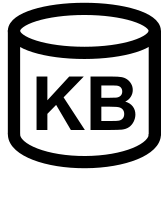
\includegraphics{KB-symbol.png}}}}
\newcommand*\KBsmall{\vcenter{\hbox{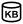
\includegraphics{KB-symbol2.png}}}}
\newcommand*\NN{\vcenter{\hbox{
\includegraphics{NN-symbol.png}}}}
\newcommand*\Graph{\vcenter{\hbox{\includegraphics{../graph-symbol.png}}}}
\newcommand*\Hypergraph{\vcenter{\hbox{\includegraphics{../hypergraph-symbol.png}}}}
\newcommand*\Tree{\vcenter{\hbox{\includegraphics{../tree-symbol.png}}}}
\newcommand*\NewSym[1]{\vcenter{\hbox{\includegraphics{#1}}}}
\newcommand{\dashh}{\textemdash~}
\newcommand{\english}[1]{\mbox{\textit{#1}}}
\newcommand{\tab}{\hspace*{2cm}}

% ***** Boxed variables inside math equations
% \newcommand*{\boxedcolor}{black}
\makeatletter
% \renewcommand{\boxed}[1]{\textcolor{\boxedcolor}{%
% \fbox{\normalcolor\m@th$\displaystyle#1$}}}
% \setlength{\fboxsep}{1pt}
\renewcommand{\boxed}[1]{\fbox{\m@th$\displaystyle\scalebox{0.9}{#1}$} \,}
\makeatother

\overfullrule=0mm

\newsavebox{\MyName}
\savebox{\MyName}{
\includegraphics[scale=0.6]{YKY.png}}

\title{\cc{神经网络中直接注入知识}{Direct knowledge injection into neural networks}}
%\normalsize{-- a minimalist cognitive architecture combining\\
%reinforcement learning and deep learning}}
\titlerunning{Direct knowledge injection}
\author{\usebox{\MyName} (King-Yin Yan)
% \\ \footnotesize{General.Intelligence@Gmail.com}
%\and
%Ben Goertzel
%\and
%Juan Carlos Kuri Pinto
}
\institute{General.Intelligence@Gmail.com}
\date{\today}

\begin{document}
\let\labelitemi\labelitemii

\maketitle

\noindent
\makebox[\linewidth]{\small \today}

\setlength{\parindent}{0em}
\setlength{\parskip}{2.8ex plus0.8ex minus0.8ex}
% \setlength{\parskip}{2.8ex}

\begin{abstract}
\cc{
	在人工智能历史上,迄今为止仍未有一个快速的学习算法,可以同时「像教孩子那样」直接注入知识。 经典逻辑 AI 可以直接写入知识,但其学习算法太慢。 深度神经网络的学习算法很快,但它是「黑盒」。 本文提出一个解决方案: 让神经网络直接作用在它自身的 weights 上。
}{
	An intelligent agent needs the ability to access its own knowledge, which comes for free in classical logic-based AI, but neural networks are notorious for the ``black-box'' problem.  The solution is to have the network act on its own weights.
}
\end{abstract}

%\begin{keywords}
%reinforcement learning, control theory, deep learning, cognitive architecture
%\end{keywords}

\setcounter{section}{-1}
\section{Introduction}

本文提出的 AGI architecture 揉合了三个结构:
\renewcommand\labelenumi{(\theenumi)}
\begin{enumerate}
	\item \textbf{reinforcement learning} (RL)
	\item classical \textbf{logic-based AI} (LBAI)
	\item \textbf{deep neural network} (DNN)
\end{enumerate}
其中 (1) 是 智能系统 根据 奖励 学习的架构,这架构本身并没有什么内容,单靠它学习人类水平的智能,会太慢,所以要加入 (2) 的结构。 而 (3) 是目前为止最有效率的机器学习算法,它本身不是 AGI 的内在结构,我们只是将它应用到 AGI 系统的关键部分。 

以下分述这三个成份。

\section{Deep neural network}

首先讲讲 神经网络。  它只是一个技术,它不是 AGI 内在的结构,我们只是将它应用到 AGI 上。  So let us first get this out of the way.

所谓 神经网络 就是:


\section{Reinforcement learning}



\section{Logic-based AI}

这部分是最复杂的结构,也是一般数学研究者比较不熟悉的。  


\cc{
智能系统需要有能力读/写它内部的知识。  例如说,一个比较蠢的智能系统可以用 sequence-to-sequence 的方式将中文翻译成英文: 
\begin{equation}
\mbox{``}\boxed{中文句子}\mbox{''} \stackrel{\vect{F}}{\longrightarrow} \mbox{``}\boxed{英文句子}\mbox{''}
\end{equation}
}{
An intelligent agent needs the ability to \textbf{access} (read or write) the contents of its knowledge base.  For example, a dumber agent may use the ``sequence-to-sequence'' technique to translate Chinese sentences into English:
\begin{equation}
\mbox{``}\boxed{Chinese sentence}\mbox{''} \stackrel{\vect{F}}{\longrightarrow} \mbox{``}\boxed{English sentence}\mbox{''}
\end{equation}
}
\cc{
$\vect{F}$ 代表系统的函数。  但系统并不真的明白句子的意义,句子只是「水过鸭背」地流过系统。 一个更聪明的系统是: 句子可以\textbf{进入}到 $\vect{F}$ 里。
}{
$\vect{F}$ is the system's \textbf{function}.  But the system does not truly understand the sentences' meaning;  The sentences simply ``pass through'' the system.  A more intelligent agent would allow sentences to \textbf{go into} $\vect{F}$.
}

%\cc{
%「内省」亦有 meta-reasoning 的意思,亦即除了\textbf{外在}的知识,系统还拥有关於系统\textbf{自身状态}的知识。 但本文中「内省」是指存取「普通知识」的能力。
%}{
%``Introspection'' also connotes \textbf{meta-reasoning}, which means that, in addition to \textbf{extrinsic knowledge}, the system also possesses knowledge about \textbf{its own states}.  In this paper, we only concern ourselves with the agent's access to extrinsic knowledge.
%}

\section{Applications}

DKI (direct knowledge injection) is useful in:
\begin{itemize}
	\item learning by instructions, or ``learn by being told'' \\
	(a technique crucial to accelearating the learning of human knowledge)
	\item belief revision / truth maintenance \\
	(the most challenging and highest-level task in logic-based AI)
\end{itemize}

\cc{
举例来说,小孩子的行为是由他内部的知识决定的,「知识决定行为」。
\begin{itemize}
	\item 当小孩子看到一个成人做的动作,他会模仿那动作。
	\begin{equation}
	\vcenter{\hbox{
\includegraphics[scale=0.5]{imitation.jpg}}}
	\end{equation}
	\item 或者小孩子听到一句说话:「不要吃污糟食物」,他明白了那句说话的意思而改变行为。
	\item 或者「今天高考放榜了,这本教科书可以丢进垃圾桶」,这句话应该由 working memory $\vect{x}$ 进入到 $\KB$ 里面,影响日后的行为(eg,以后不会再见到那本书)。 
\end{itemize}
}{
For example, a child's behavior is determined by his internal knowledge; ``Knowledge determines action''.
\begin{itemize}
	\item When a toddler watches an adult's gesture, he tries to imitate that gesture:
	\begin{equation}
	\vcenter{\hbox{
\includegraphics[scale=0.5]{imitation.jpg}}}
	\end{equation}
	\item Or when a child hears a saying:  ``don't eat dirty food'', he understands the words and changes his behavior.
	\item Or, ``today I graduated from university, no more exams from now on.''  This sentence in work memory $\vect{x}$ should enter into $\KB$ so it would influence subsequent behavior.
\end{itemize}
}
\cc{
这些例子都涉及到将「感觉资料」放进 $\vect{F}$ 里面:
}{
Both examples involve putting ``sensory data'' into $\vect{F}$:
}
\begin{equation}
\boxed{sensory data} \hookrightarrow \vect{F}
\end{equation}

\section{Cartesian closure}

在数理逻辑中,\textbf{命题逻辑}和\textbf{一阶逻辑}、\textbf{高阶逻辑}之间存在一个 gap。  一般来说,数学家比较熟悉命题逻辑,因为它等价於很多在传统数学中常见的结构例如 Boolean algebra 等。  在 \textbf{拓樸} 中,$\cup$ 和 $\cap$ 对应於 $\vee$ 和 $\wedge$,所以 拓扑 也可以看成是 逻辑 的一种形式。  另外,我们熟悉的 \textbf{Bayesian network} 也是命题逻辑的扩充,亦即在命题上附加了 \textbf{概率}。 然而,一阶逻辑的结构比较麻烦,在数学上是较偏门的课题。  用计算机科学的术语,将命题逻辑的技巧转移到一阶逻辑,这动作叫 ``lifting'',於是会产生例如 first-order Bayesian network 这类较复杂的东西,而高阶逻辑则更复杂。  注意: 命题逻辑的复杂性是 NP-complete 的范围,但高阶逻辑的复杂性是 undecidable 的,因为高阶逻辑可以做 Turing machine 的所有工作,而 halting problem 是 undecidable 的。 
\begin{equation}
\vcenter{\hbox{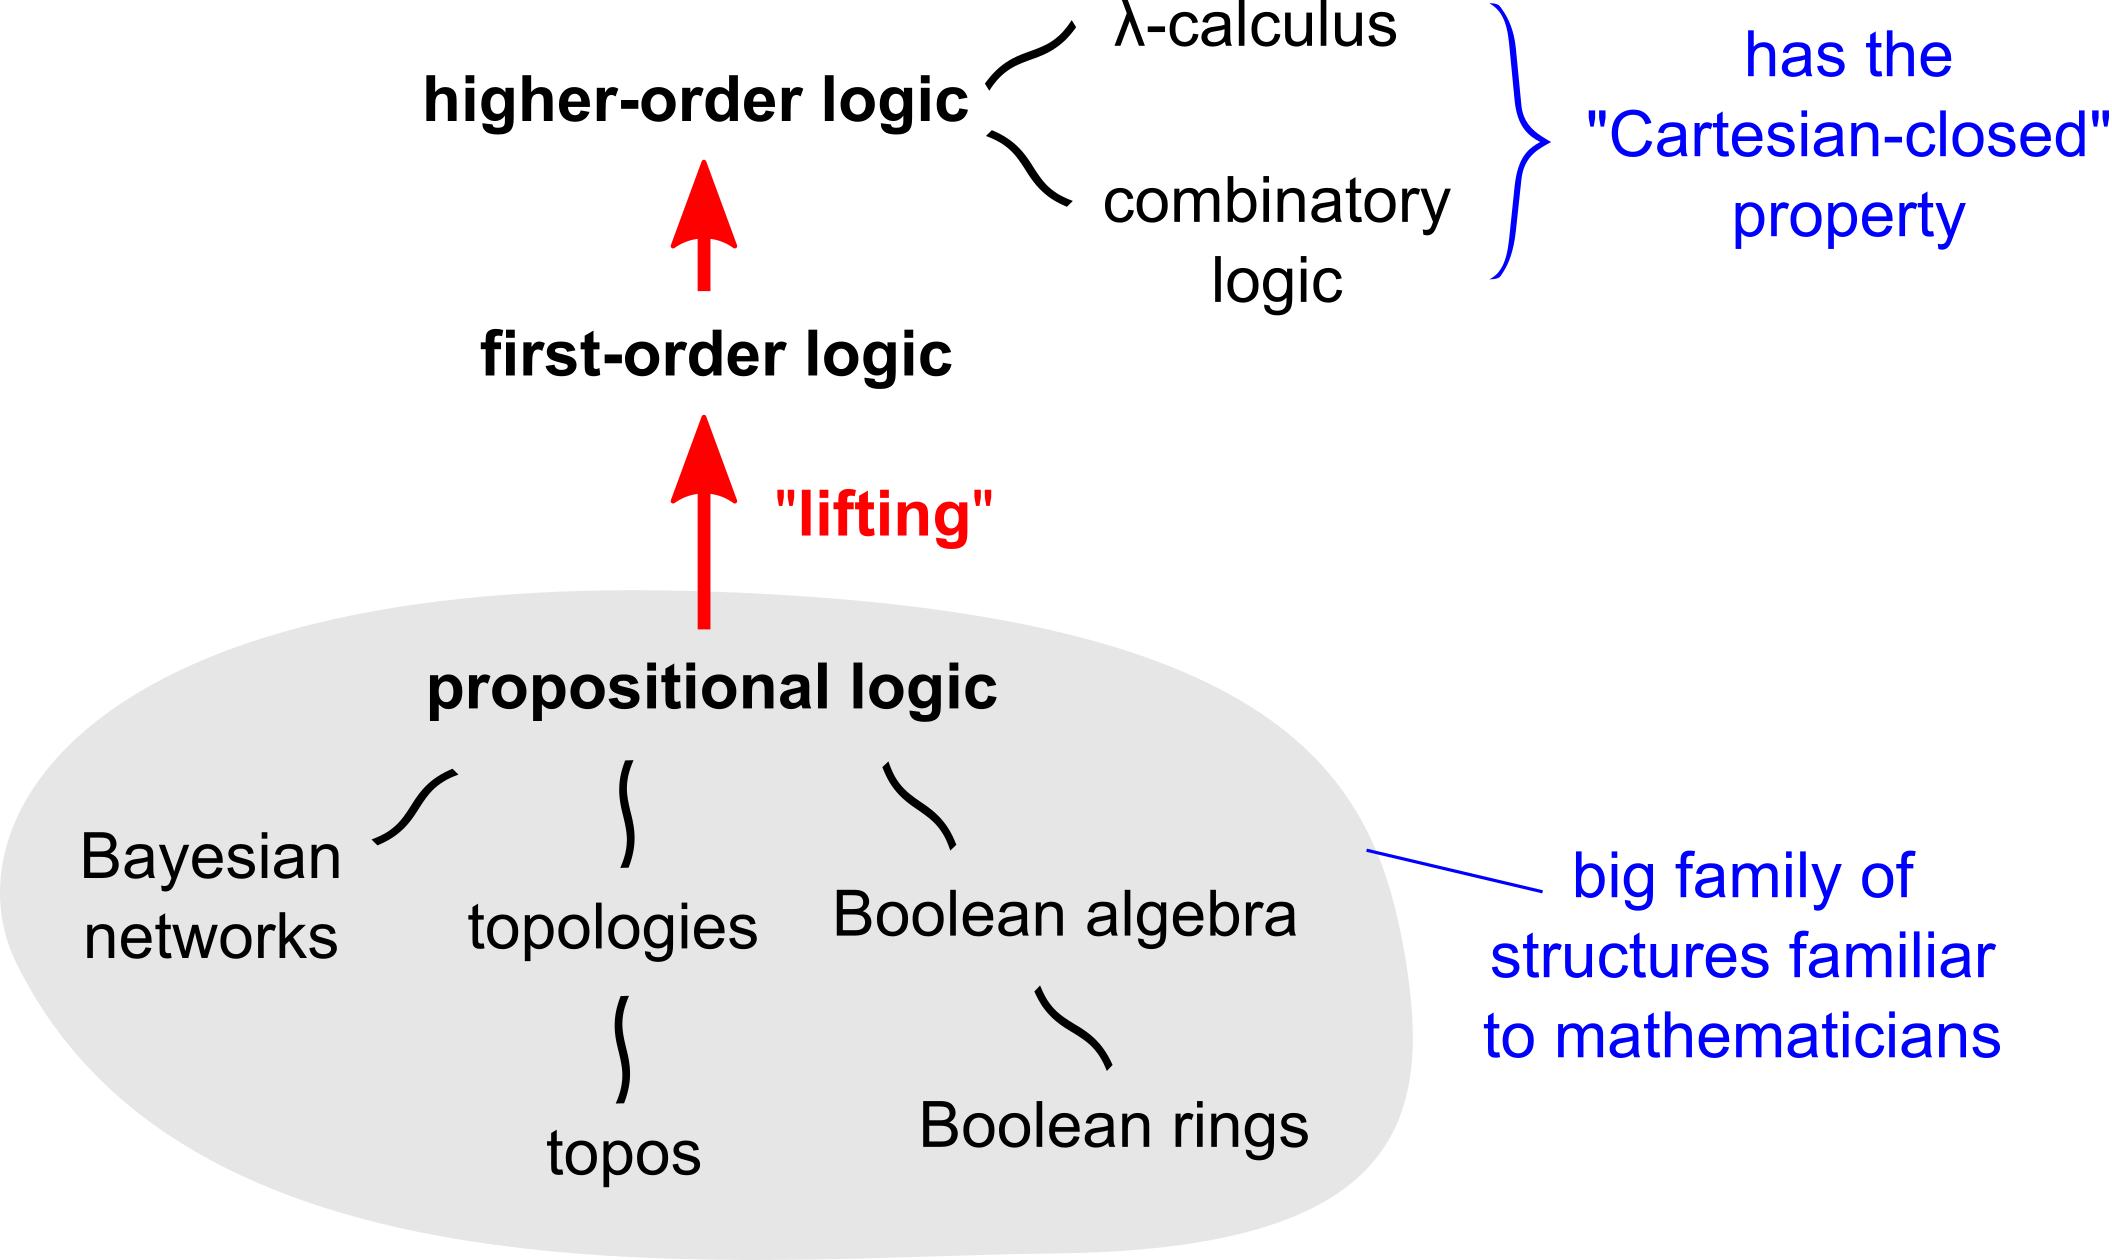
\includegraphics[scale=0.7]{logic-lifting.png}}}
\end{equation}
\uline{在人工智能中,我们必须用到 一阶逻辑 或以上},因此 lifting 是一个很头痛的问题。 高阶逻辑的 ``power'' 似乎来自於一个特性,即 Cartesian-closure,它是高阶逻辑的本质。

Cartesian-closed 是指在某个範畴内,对任意的 $A,B$,都必然可以找到它们的:
\begin{equation}
\boxed{\mbox{product}} \; A \times B \quad \mbox{和} \quad B^A \; \; \boxed{\mbox{exponentiation}} 
\end{equation}
在逻辑中这对应於:
\begin{equation}
A \wedge B \quad \mbox{和} \quad A \rightarrow B
\end{equation}

DKI requires the functional closure $\mathbb{X} \simeq \mathbb{X}^{\mathbb{X}}$ which yields a \textbf{Cartesian-closed category} (CCC).

\cc{
举例来说,「吃了污糟的食物会肚痛」是一个句子,它经由 $\NewSym{eye-symbol.png}$ 进入 mental state $\vect{x}$ ,变成 proposition。 但我们希望这逻辑命题变成 $\KB$ 的一部分。 
}{
For example, ``eating dirty food causes stomach pains'' is an NL sentence, it enters from $\NewSym{eye-symbol.png}$ into the mental state $\vect{x}$, as a \textbf{proposition}.  But we want $\vect{x}$ to become part of $\KB$.  
}
$\vect{F}$ is the state-transition function:
\begin{equation}
\vect{x}_{n+1} = \vect{F}(\vect{x}_n)
\end{equation}
where \\
\tab $\vect{F} = \KB = \NN$ \\
\tab $\vect{x} = $ state

An individual logic rule is a \uline{restriction} of $\vect{F}$ to a specific input;  Perhaps I could call such elements ``micro-functions''.

$\vect{F} \equiv \KB$ is the \uline{``union'' of micro-functions}:
\begin{equation}
\KB = \biguplus \vect{f}_i
\end{equation}
At this point the meaning of $\biguplus$ is unspecified yet.  $\vect{F}$ is the sum total of objects like $\vect{x}$:
\begin{equation}
\vect{F} = \biguplus \vect{x}_i
\end{equation}
\cc{
但 $\vect{F}$ 是一个神经网络,它的一般形式是:
}{
But $\vect{F}$ is a neural network;  Its general form is:
}
\begin{equation}
\boxed{output} \; \vect{x}_{n+1} = \vect{F}(\vect{x}_n) = \sigmoid \stackrel{1}{W} \; \sigmoid \stackrel{2}{W} \; ..... \; \sigmoid \stackrel{L}{W} \; \vect{x}_n
\end{equation}
$L$ = total number of layers.  
\cc{
由於各层的非线性「纠缠在一起」,表面上无法将神经网络「分解」。 直到笔者受了 David Ha \textit{et al} 提出的 PathNet \citep*{Fernando2017} 理论所启发,PathNet 是由一些较小的神经网络 modules 组成,所以或许可以建构如下形式的「丝状神经网络」:
}{
Because all the layers of non-linearities are ``entwined together'', apparently we cannot ``decompose'' a neural network.  That is, until the author hears of David Ha \textit{et al}'s PathNet \citep*{Fernando2017} idea, which is a big network consisting of smaller neural-network modules.  Inspired by that, I propose to construct a ``threaded'' neural network:
}
\begin{equation}
\vcenter{\hbox{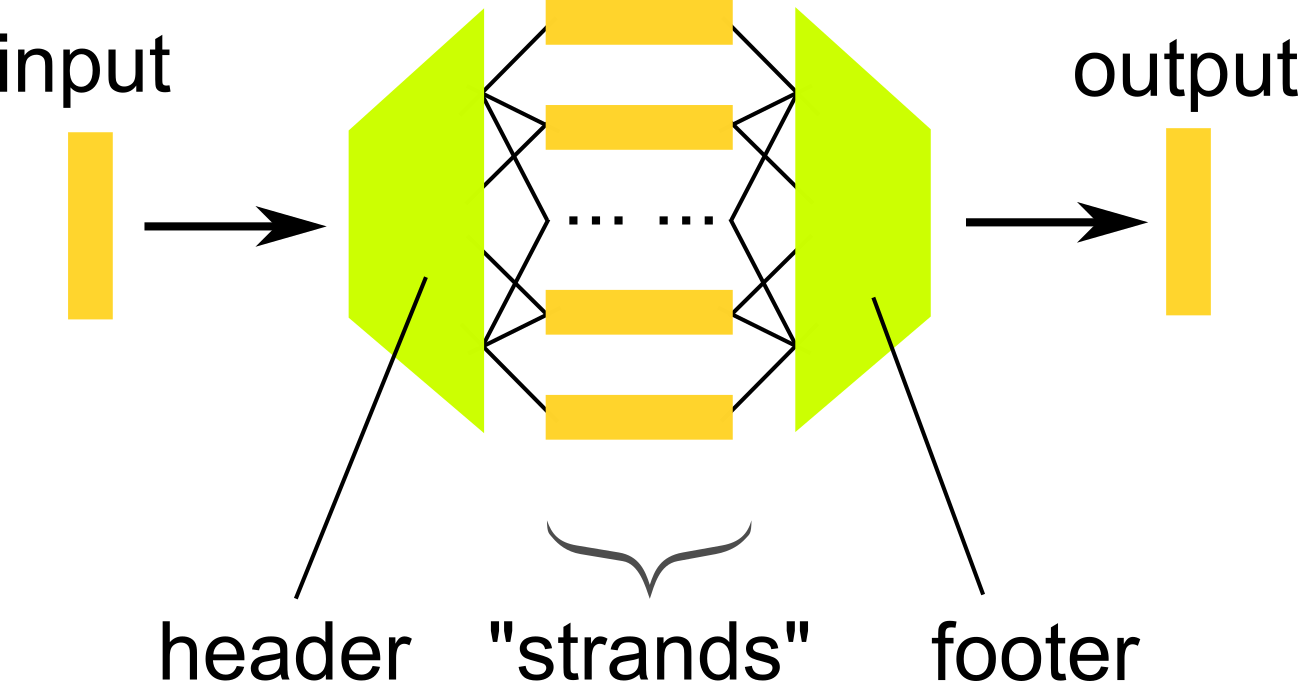
\includegraphics[scale=0.75]{reticular-NN.png}}}
\end{equation}
\cc{
这些「丝条 $\NewSym{strand.png}$」可以是简单的神经网络,例如每个的宽度或深度很小,因而可以用较短的 weights vector 描述。  正是因为这原因,一个 $\NewSym{strand.png}$ 本身可以作为神经网络的输入。 但整个神经网络 $\vect{F}$ \uline{无法输入自己},因为根据 Cantor's theorem,$\mathbb{X} = \mathbb{X}^{\mathbb{X}}$ 是不可能的。
}{
These ``strands'' $\NewSym{strand.png}$ are simpler neural networks, for instance with smaller widths and depths, so they can be described by shorter weight vectors.  Precisely for this reason, a  $\NewSym{strand.png}$ can be presented as input to its own neural network.  We  \uline{cannot pass the entire network $\vect{F}$ to itself}, due to Cantor's theorem, which says $\mathbb{X} = \mathbb{X}^{\mathbb{X}}$ is impossible.
}

Let $\overline{\vect{F}} = \NewSym{header.png} $ header, $\underline{\vect{F}} = \NewSym{footer.png} $ footer, $\vect{f}_i = \NewSym{strand.png}$ strands, then (abusing the $\biguplus$ notation):
\begin{equation}
\vect{F} = \overline{\vect{F}} \circ \biguplus \vect{f}_i \circ \underline{\vect{F}}
\end{equation}
\cc{
每个 $\NewSym{strand.png}$ 大约对应於逻辑上的一个\textbf{命题}(proposition, 可以是条件命题或普通命题)。
}{
Each $\NewSym{strand.png}$ roughly corresponds to a single \textbf{proposition} in logic-based AI. Such propositions may be conditional or plain statements.
}

读者或许会质疑,这个「条状」结构为什么一定要设计成这样?  其实我也觉得这个设计不够 elegant,甚至不太肯定它会不会 work。  在 \S\ref{decomposition-of-F} - \S\ref{spectral-compression} 我们会介绍一个数学上更优美的做法。 

%\section{Structure of memories}
%
%The ``main memory'' $\vect{F}$ can take the form of a tree ($\Tree$), graph ($\Graph$), or hyper-graph ($\Hypergraph$), with increasing complexity.
%
%The \textbf{mental state} $\vect{x}$, or ``working memory'', can also assume the above-mentioned forms.
%
%Currently I am not sure whether to place \textbf{episodic memory} inside $\vect{F}$ or as a separate module outside $\vect{F}$.
%
%We need to organize the $\NewSym{strand.png}$'s in the form of $\Tree$, $\Graph$ or $\Hypergraph$, in such a way that the resulting structure is also a neural network, or more generally a mathematical \textbf{function} in Hilbert space.
%
%But there is one simple way:  Basically, a deep network is automatically ``tree-like'' because of its many layers (\textbf{levels}) of weights organized hierarchically.  Thus we can build a network like this:
%\begin{equation}
%\vcenter{\hbox{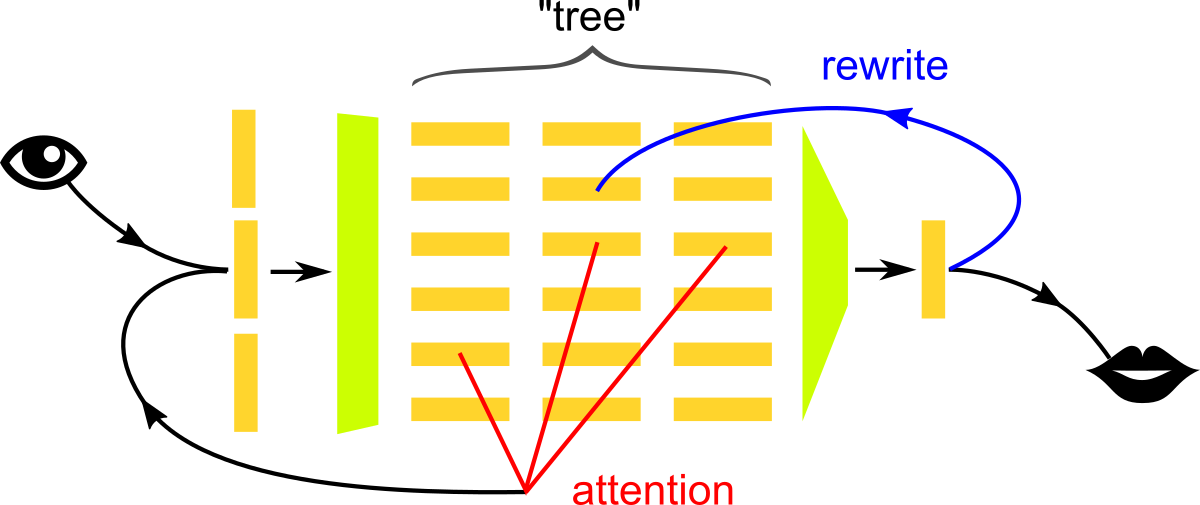
\includegraphics[scale=0.7]{introspection-tree-bank.png}}}
%\end{equation}
%The {\color{red}attention mechanism} selects a number of $\NewSym{strand.png}$'s to be the \textbf{current state} or ``working memory''.  Notice that the input size is bigger than the output size, which reflects the structure of the logical \textbf{consequece operator} $\vdash$.

\section{Overall architecture}

For reference, the architecture for \textbf{visual recognition} is:
\begin{equation}
\vcenter{\hbox{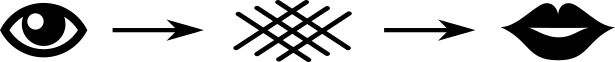
\includegraphics[scale=0.6]{vision-architecture.png}}}
\end{equation}
Our basic AGI architecture is:
\begin{equation}
\vcenter{\hbox{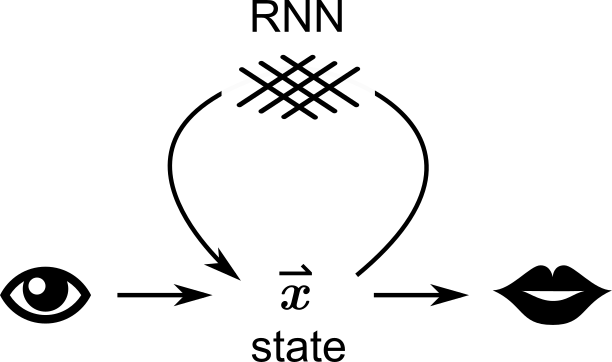
\includegraphics[scale=0.6]{basic-architecture.png}}}
\label{basic-arch}
\end{equation}

$\NN$ = [deep] neural network, trained via \textbf{reinforcement learning}

The overall \textbf{recurrent} setup operates like this:
\begin{equation}
\vcenter{\hbox{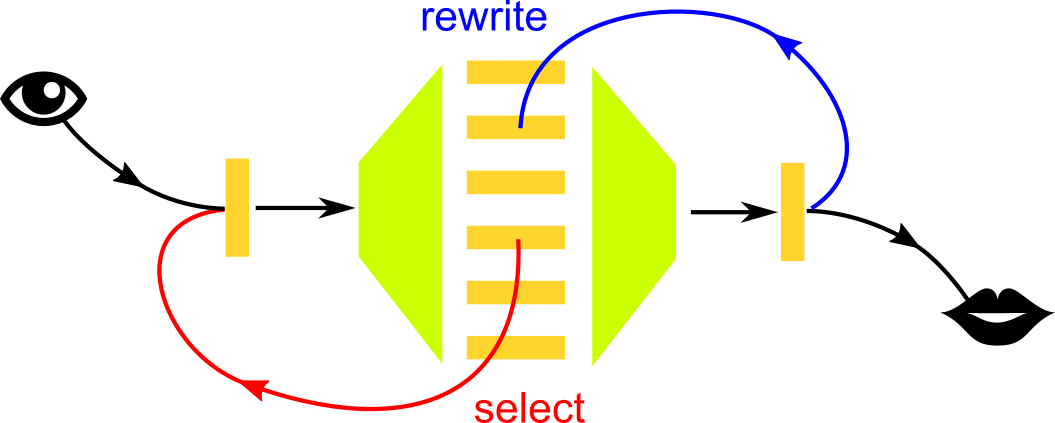
\includegraphics[scale=0.7]{introspection-simple.png}}}
\end{equation}
注意: $\NewSym{eye-symbol.png}$ 的原始输入不可以直接写入 $\NewSym{strand-vertical.png}$,因为 $\NewSym{strand-vertical.png}$ 会变成 $\NewSym{strand.png}$ = weights,而直接写 weights 的后果当然是灾难性的。  换句话说,$\NewSym{strand.png}$ 的结构是要用 emergent(涌现)的方法 learn 出来,不能被外界的输入干扰。  $\NewSym{eye-symbol.png}$ 和 $\NewSym{mouth-symbol.png}$ 的输入/输出要透过某些神经网络的 mapping 间接地做。

Viewing the ``information flow'' in a simplified way, we notice a ``second'' pass through the network's internal weights:
\begin{equation}
\vcenter{\hbox{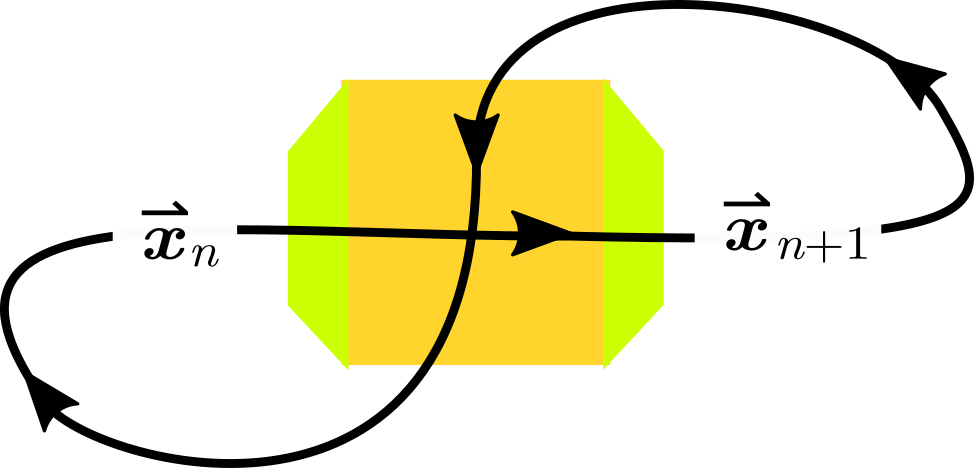
\includegraphics[scale=0.5]{introspection-flow.png}}}
\end{equation}
\cc{
这种操作上的结构在经典逻辑 AI 是「免费赠品」,但似乎还未有人提出过神经网络的做法。
}{
This operational architecture has always been a ``free gift'' in logic-based AI systems, but it seems that a neural-network implementation has not been proposed before.
}

对应於经典逻辑 AI:
\begin{equation}
\NewSym{IRNN.png} = \KB 
\end{equation}
\begin{itemize}
	\item The \textbf{horizontal pass} represents using the $\KB$ for logical inference (thinking), ie:
	\begin{equation}
	\vect{x}_n  \cup \KB \sststile{}{} \vect{x}_{n+1}
	\end{equation}

	\item The \textbf{vertical pass} represents reading/writing information to/from $\KB$:

	\begin{itemize}
		\item \textbf{Update:}  $\vect{x}$ 是 $\KB$ 的一部分,所以 $\vect{x}_{n+1}$ 改变了,$\KB$ 也要 update。
		
		\item \textbf{Read:}  $\vect{x} = $ working memory 会因为 \textbf{注意力} (attention) 而改变,所以 $\vect{x}_{n+1}$ 并不直接进入下一轮的 iteration,而是先经过 $\KB$ 的 \textbf{attentional change}。
	\end{itemize}

\end{itemize}

In logic-based AI this workflow has always been standard (but not made explicit):
\begin{equation}
\vcenter{\hbox{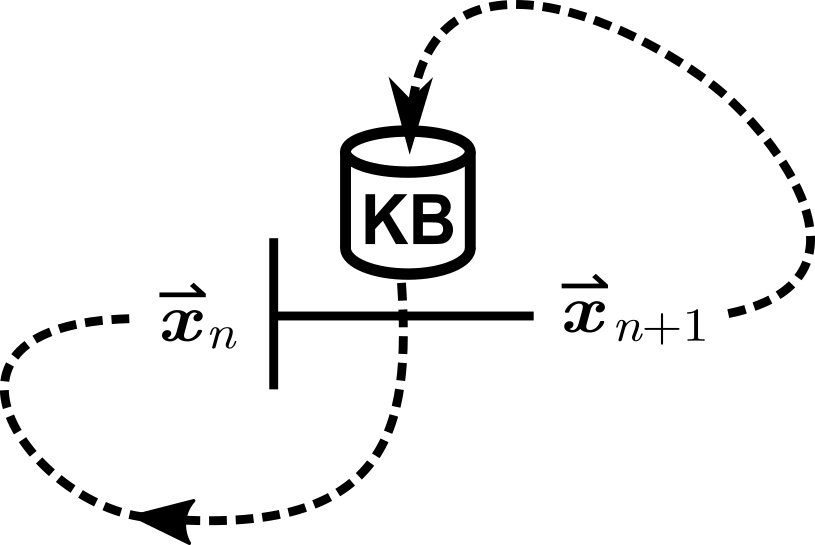
\includegraphics[scale=0.5]{introspection-flow-KB.png}}}
\end{equation}

\section{What is required of $\vect{F}$?}
\label{decomposition-of-F}

We now try to explain the meaning of
\begin{equation}
\vect{F} = \biguplus \vect{x}_i
\end{equation}
Our goal is to organize the $\NewSym{strand.png}$'s into a deep network.  What are the most general \textit{desiderata} for such a function $\vect{F}$?
\begin{enumerate}

	\item $\vect{F}(\vect{x}; \vect{\theta})$ is a function of $\vect{x}$ parametrized by $\vect{\theta}$.
	
	\item the parameters $\vect{\theta}$ is organized hierarchically with the ``deep'' property,\\
	ie, high-level $\vect{\theta}_i$'s have higher ``degree''.
	
	\item $\vect{F}(\vect{x}; \vect{\theta})$ is capable of universal function approximation.
	
	\item $\vect{x}$ can be put into $\vect{\theta}$, ie, $\vect{\theta}$ is a collection of $\vect{x}$'s.
	
	\item $\vect{F}$ encodes \textbf{logical consequence}.
	
\end{enumerate}
The last condition (F5) is hardest to satisfy, but there is an informal argument that may justify it.  For example, suppose:
%\begin{equation}
\begin{align}
&\vect{x\vect{}} = \mbox{``\textit{all men are mortal}''} &\quad\quad& \mbox{is put into } \vect{F} = \KB. \nonumber \\
&\vect{x}_0 = \mbox{``\textit{Socrates is a man}''} &\quad\quad& \mbox{is the new input.} \nonumber \\
&\mbox{Then the expected output should be:} && \\
&\vect{F}(\vect{x}_0) = \mbox{``\textit{Socrates is mortal}''} &\quad\quad& \nonumber
\end{align}
%\end{equation}
凭什么认为 $\vect{F}$ 能满足类似上面的要求?  可以将一个 conditional proposition 看成是一个 mapping,它将 source domain $\mathbb{X}$ 的某个区域映射到 target domain(也是 $\mathbb{X}$)的某个区域,例如: 
\begin{equation}
\vcenter{\hbox{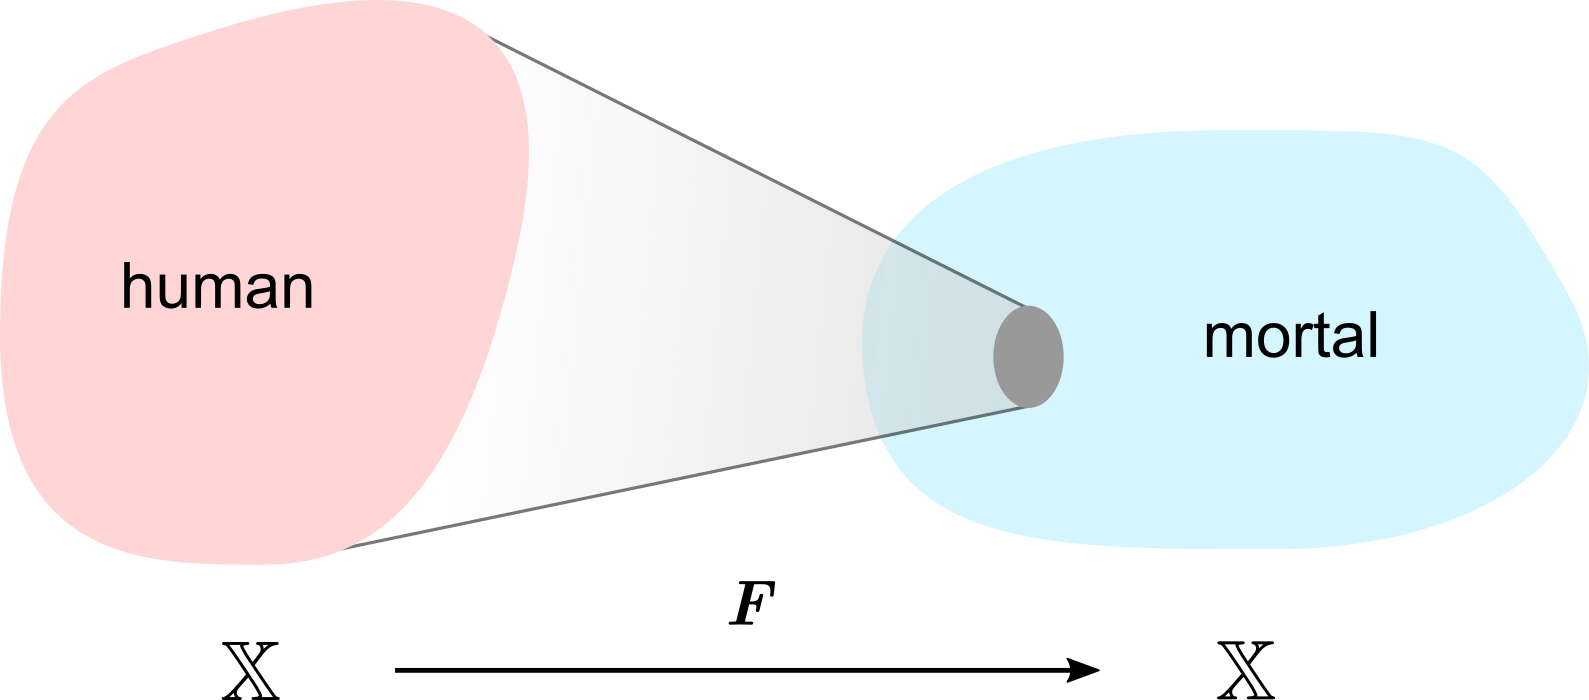
\includegraphics[scale=0.7]{F-as-a-mapping.png}}}
\end{equation}
\cc{
	而我们有信心 $\vect{F}$ 能够表达这个 mapping 的原因,正如在机器视觉中,类似的 $\vect{F}$ 里面有些神经元可以辨认「眼、耳、口、鼻」等 features,原理是一样的。 换句话说,「X是人 $\rightarrow$ X会死」这句条件命题,其实和负责辨认「眼」这个 feature 的那些神经元,本质上是没有分别的。 
}{
	If we look at $\vect{F}$ as a deep network for visual recognition, some mid-level ``features'' such as ``eye'', ``nose'', ``mouth'' etc may be recognizable by $\vect{F}$, and we may surmise that each feature is associated with a local cluster of weights.  
}

\section{Decomposition of $\vect{F}$}

回顾一下: 经典 AI 中,$\KB$ 装著一堆 logic formulas,我们可以直接写入/读出它们。  但现在 $\KB$ 变成了一个函数 $\vect{F}$,那些 逻辑法则 隐藏在 $\vect{F}$ 这个 mapping 里面,需要某种方法将它「分解」。

换句话说,我们需要的是将 $\vect{F}$ 分拆成一些小部分,亦即是 $\vect{F}$ 对於某个输入 $\vect{x}$( 及其邻域)的 \textbf{截面} (section, or restriction)。  假设获得了这些截面函数之后,我们再需要一个方法,将一个截面「放进」$\vect{F}$ 里面。
\begin{equation}
\vcenter{\hbox{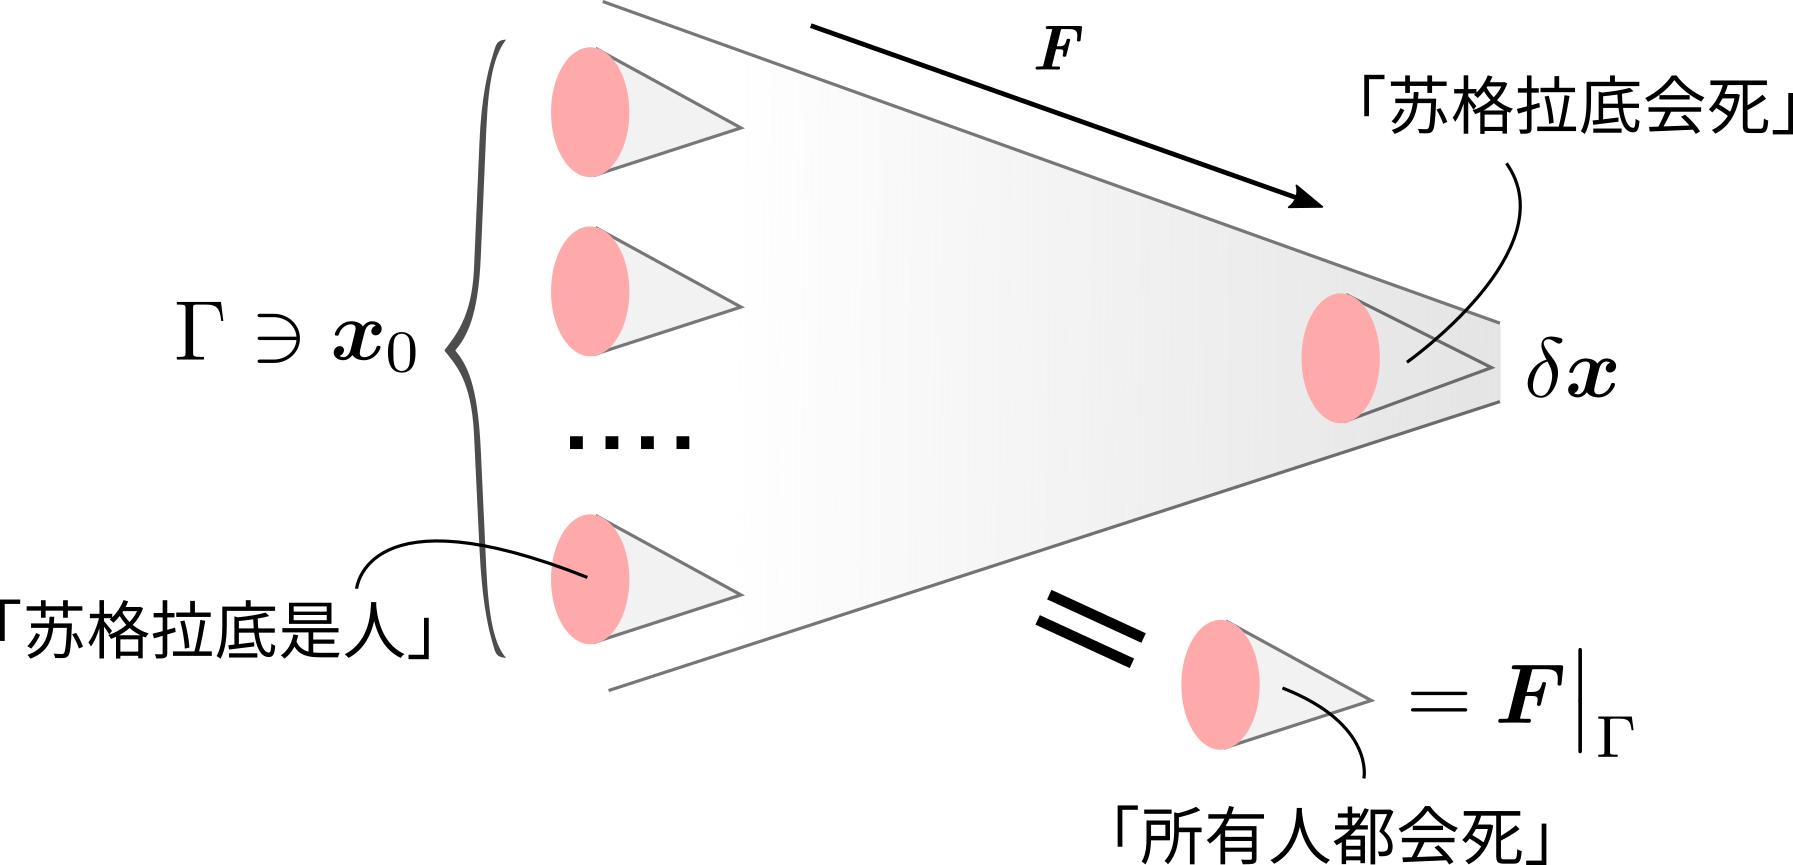
\includegraphics[scale=0.7]{F-as-a-mapping-2.png}}}
\end{equation}
$\vect{x_0}$ = current state,它由若干个 $\NewSym{single-proposition-as-map.png} = $ \textbf{命题} 构成。

(要透彻理解上面这幅图,需要熟悉命题逻辑和谓词逻辑的几何化,这在我较早前的论文 \citep{YanBridge} 有讲述。 那篇论文有些细节需要更新,但基本要点没变。)

$\delta \vect{x}$ 的意思是指,将当前状态由 $\vect{x}$ 改写成 $\vect{x} + \delta \vect{x}$。  换句话说,原本设定的是 $\vect{F}: \vect{x} \mapsto \vect{x}'$,但实际上我们 implement 的是 $\vect{F}: \vect{x} \mapsto \delta \vect{x}$。 因为逻辑中 $\vdash$ 的特性是它 \uline{每次只改变一个(或少数的)命题}。  这也是一种 restriction,即原本 ``free'' 的函数空间变成某个 subspace。

经过 update: $\vect{x}_0' = \vect{x}_0 + \delta \vect{x}$ 之后,$\vect{x}_0'$ 也会「忘记」它里面的一个/几个命题,保持 $\vect{x}$ 的长度不变。

更重要的是: \uline{$\vect{F}$ 的 restriction 也是一个命题}。  换句话说,图中的大三角形也是一个 $\NewSym{single-proposition-as-map.png}$。  它将 $\vect{x}_0$ 的\textbf{邻域} $\Gamma$ 映射到 $\delta \vect{x}$, 而 $\vect{x}_0$ 本身也是由其他 $\NewSym{single-proposition-as-map.png}$ 组成的。  这 restriction 记作 $\vect{F}|_{\Gamma}$。 

(下一步会将 $\delta \vect{x}$ 放进 $\vect{F}$ 里,但 $\delta \vect{x}$ 这个函数的 source 邻域并不是 $\Gamma$。 这些细节初读时可以不理。)

\subsection{「责任集」(``responsible set'')}

但是,当 $\vect{F}$ 是一个神经网络时,怎样获得「截面」? 

$\vect{F}$ 这个 mapping 是由它的 parameters 决定,亦即 weights。  当输入 = 某个 $\vect{x}_0$ 时,每个 weights 的贡献不同,只有一个 subset of weights「负责」这个截面的输出,我将这个 subset 称作「责任集」(responsible set)。 

我的想法是受到 TensorFlow Playground 的这图片启发的:
\begin{equation}
\vcenter{\hbox{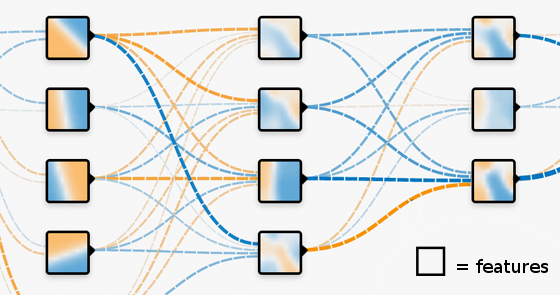
\includegraphics[scale=0.5]{TensorFlow-visualization.png}}}
\end{equation}
可以看到 weights 的大小不同,它们对函数 $\vect{F}$ 在输入 $\vect{x}_0$ 的贡献也不同。  What we need is the \uline{set of weights activated by the specific input $\vect{x}_0$}, in other words, they are the set of \textbf{outputs} (or ``activities'') of all neurons.  Let's denote it as $\vect{W}(\vect{x})$.

后来我发现了 [Courbariaux, Bengio, \& David 2015] 提出的 ``BinaryConnect: training deep neural networks with binary weights'' \citep{Courbariaux2015},他们指出,可以将 weights 限制为 $\{ -1, 1 \}$ 两个值,但 gradients 仍然保持 precision,这种神经网络仍然有 state-of-the-art 的表现。 

\subsection{Compression}
\label{spectral-compression}

现在问题是怎样 压缩 那责任集里面的 weights。  Joseph Cheng 提议用 auto-encoder,似乎是一个很好的解决办法。 左图是典型的 auto-encoder,它的 hidden layer 较小,特徵「被逼」压缩到较小的空间。  在我们的 architecture 上加上 auto-encoder,则变成右图的「8字形 architecture」:
\begin{equation}
\vcenter{\hbox{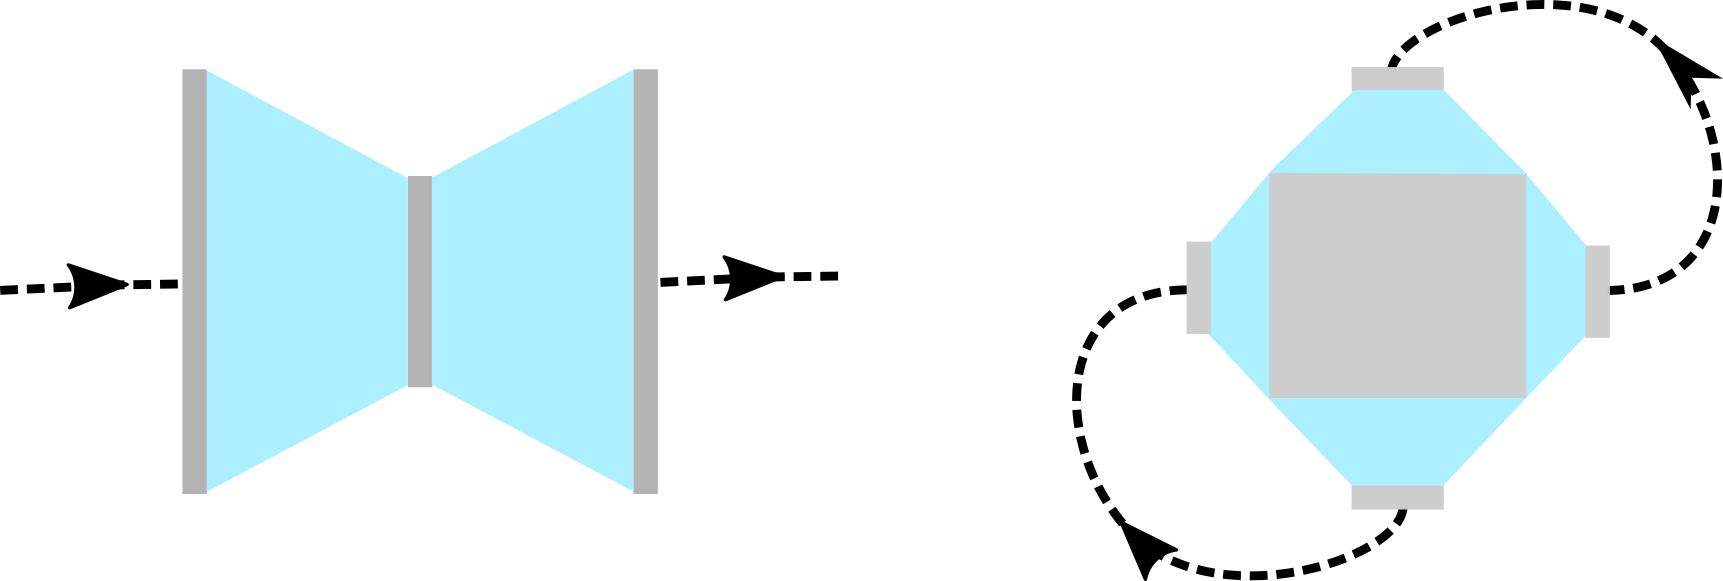
\includegraphics[scale=0.6]{auto-encoder.png}}}
\end{equation}
但有个技术上问题: 垂直方向的那个 $\NewSym{blue-NN.png}$ 网络需要连接到中央网络的所有 weights,但这些 weights 数目太多。 

Now we need a way to \textbf{compress} $\vect{W}(\vect{x})$ to prune out the low-contribution (ie, small) weights.  The Fourier (or wavelet) transform is a good candidate because it can compress $\vect{W}(\vect{x})$ to a \uline{fixed-length vector}, which can then be used as inputs to the neural network $\vect{F}$.

The compression (which is a projection, $P$) is performed via:
\begin{equation}
P \; \vect{F} = \sum_{i=1}^{N} \langle \vect{F}, \Psi_i \rangle \Psi_i
\end{equation}
where $\{ \Psi_i \}_1^N$ is the basis set.  

The Fourier sequence basis set tends to 0:
I think the implication is that, for sufficiently smooth functions, the high-frequency contributions of a Fourier sequence would tend to 0.  This means that if we chop off the sequence at some number $n$, we get an approximation, ie, compression.  However, this form of compression is weak because the error does not decay fast enough.  A better scheme is to choose the first $k$-largest coefficients;  This way, the error decays exponentially.  The price we pay is that the compression scheme is no longer \textbf{linear}, in the sense that if $\hat{f}$ and $\hat{g}$ approximate 2 signals $f$ and $g$, then the sum of the signals $(f + g)$ may no longer be approximated by $(\hat{f} + \hat{g})$.


\section{\cc{几何结构}{Geometric structure}}

[ 此段对熟悉微分几何的人或许有帮助,否则可以略过。]

首先我们有一个很 standard 的 Hamiltonian 力学系统/控制系统的结构:
\begin{equation}
\label{tangent-bundle}
\vcenter{\hbox{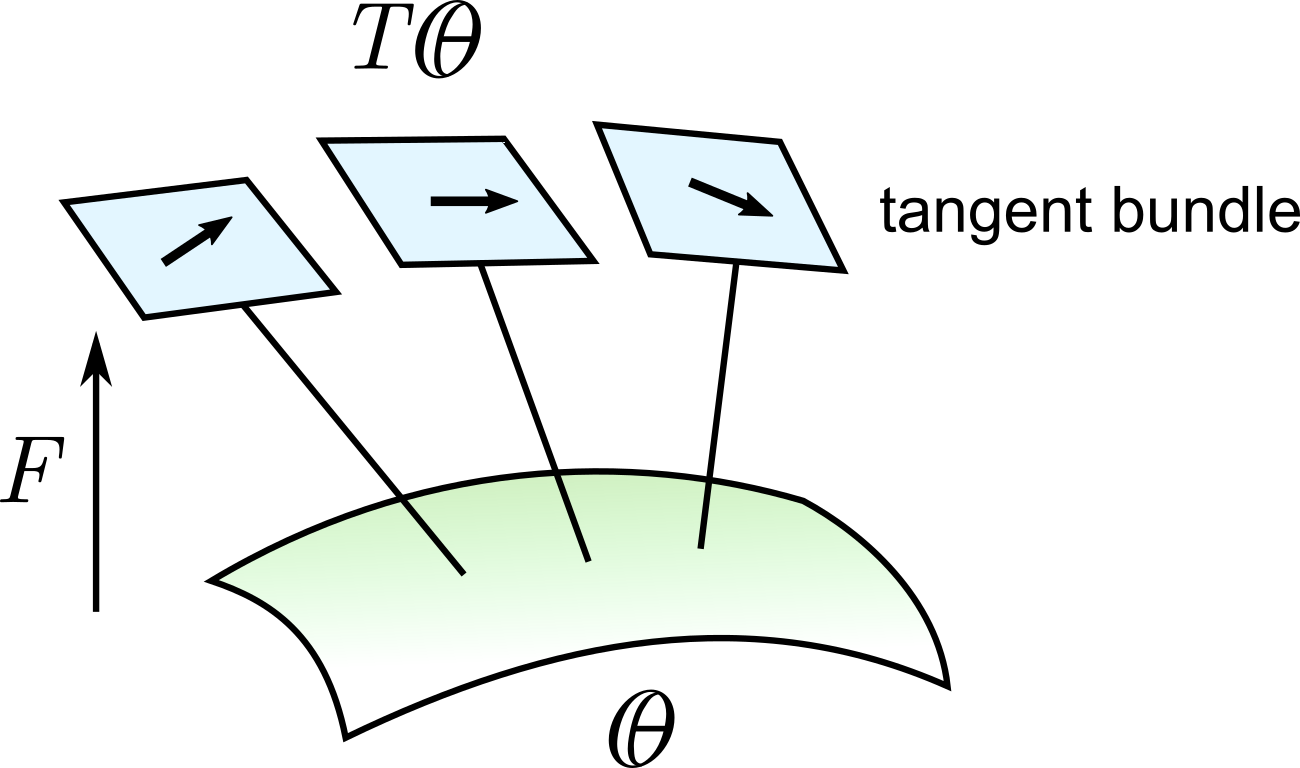
\includegraphics[scale=0.6]{tangent-bundle.png}}}
\end{equation}
$\vect{x} = \mbox{working memory} \subset \vect{\theta}$,$\vect{\theta}$ 代表整个 $\KB$ 的状态,而 $\vect{\theta} \in \NewSym{bbTheta.png}$,后者是所有可能 $\KB$ 的空间。
\begin{equation}
\dot{\vect{x}} = \vect{F}(\vect{x})
\end{equation}
是系统的\textbf{状态方程}。 换句话说,在思维空间 $\NewSym{bbTheta}$ 中的一个点就是思维状态 $\vect{x} \subset \vect{\theta} \in \NewSym{bbTheta}$,而 $F$ 给出的是这个点在\textbf{思考}过程中的的「运动速度」$= \dot{\vect{x}}$。  换句话说,$\vect{F}$ 定义了一个 vector field,它是思维空间中思维的 ``flow'',或者可以叫作「理性流」。  每个点的速度属於流形 $\NewSym{bbTheta}$ 上的 tangent space,他们的总和就是 tangent bundle。  而 tangent bundle + base manifold (亦即「位置 \& 动量」)构成系统的「相空间」(phase space)。

另外,特别地,有这个 sheaf of functions 的结构:
\begin{equation}
\label{sheaf}
\vcenter{\hbox{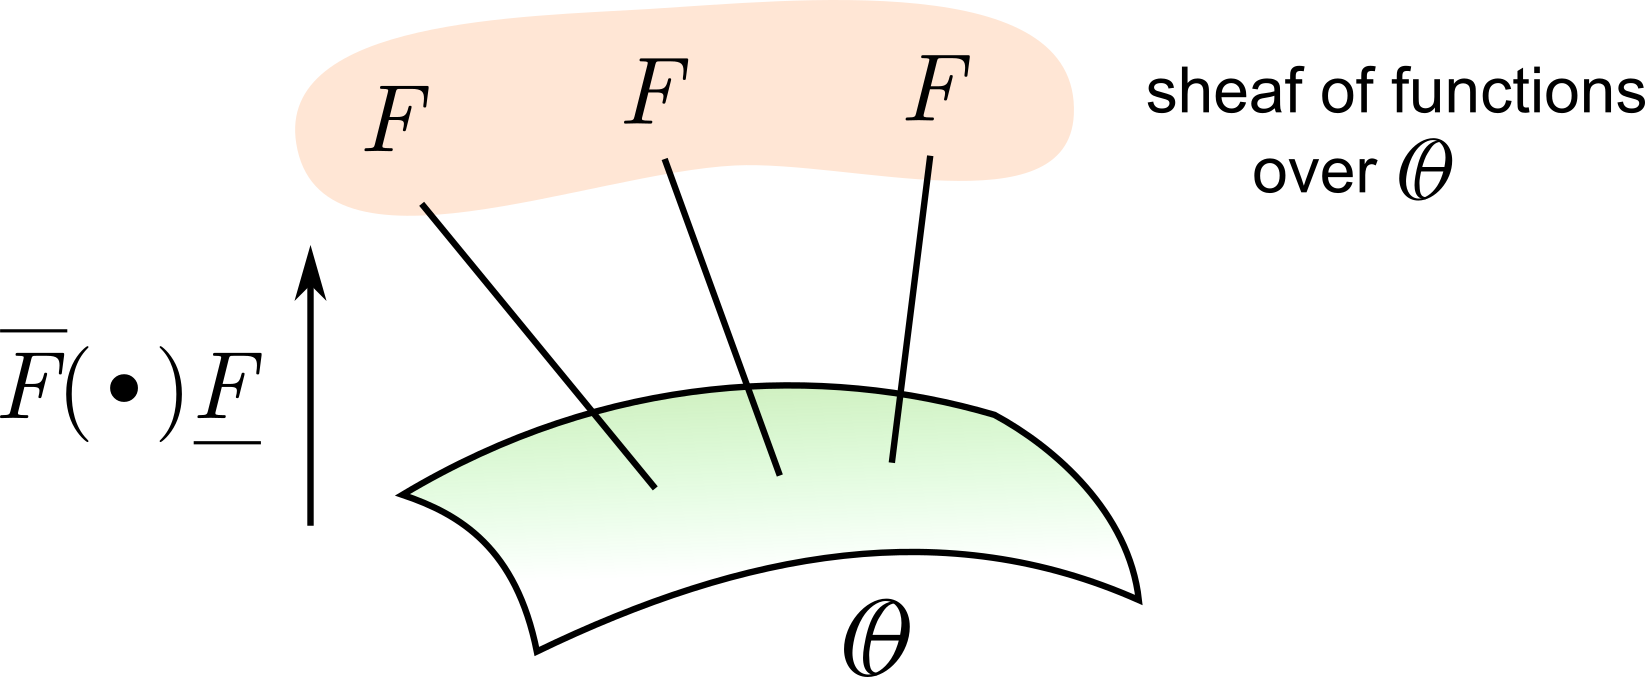
\includegraphics[scale=0.6]{sheaf.png}}}
\end{equation}
换句话说,给定 $\vect{x} \in \NewSym{bbTheta}$ ,我们可以透过
\begin{equation}
\vect{F} = \overline{\vect{F}} \circ (\vect{x} \subset \vect{\theta}) \circ \underline{\vect{F}}
\end{equation}
得出 $\vect{F}$,而这个 $\vect{F}$ 再给出对应於这点的 $\dot{\vect{x}}$。

注意 $(\ref{tangent-bundle})$ 和 $(\ref{sheaf})$ 是两个不同的结构,只是它们的 base manifold 相同。 

特别之处在於 $\vect{F}$ 是由参数 $\vect{x} \subset \vect{\theta} \in \NewSym{bbTheta}$ 确定的(因为 $\vect{x}$ 是 $\vect{\theta} = \KB$ 的一部分,而所有可能的 $\KB$ 属於思维空间 $\NewSym{bbTheta}$),换句话说:
\begin{equation}
\vect{F}(\vect{x}) \equiv \vect{F}_{\vect{\theta}}(\vect{x}) \equiv \vect{F}(\vect{x} ; \vect{\theta})
\end{equation}
这和经典控制并没有抵触,因为经典理论中,$\vect{F}$ 也是位置 $\vect{x}$ 的函数。  更确切地说,位置空间其实是由 $\vect{\theta} \in \NewSym{bbTheta}$ 决定的,$\vect{x}$ 只是 $\vect{\theta}$ 的一部分。

In general, the differential version seems to be a bad idea, as the increments of $\vect{x}$ is small, and the $\KB$ may be overwhelmed by recent memories of $\vect{x}$, which is a wasteful usage of weights.

\section{Conclusion}

其实我自己也怀疑,这个 architecture 是否太复杂了,究竟值不值得做?  而暂时我只能说,它符合了两项非常难达到的要求: 
\begin{itemize}
	\item $\KB$ is represented as a neural network (that admits a fast learning algorithm);

	\item Symbolic knowledge can be directly \textbf{injected} into $\KB$.
\end{itemize}

\section{Future direction}

There may exist some variations and improvements under this general architecture.

Another problem is the design of the \textbf{memory system}, in particular \textbf{episodic memory}.  This is the general idea, but details are still undecided:
\begin{equation}
\vcenter{\hbox{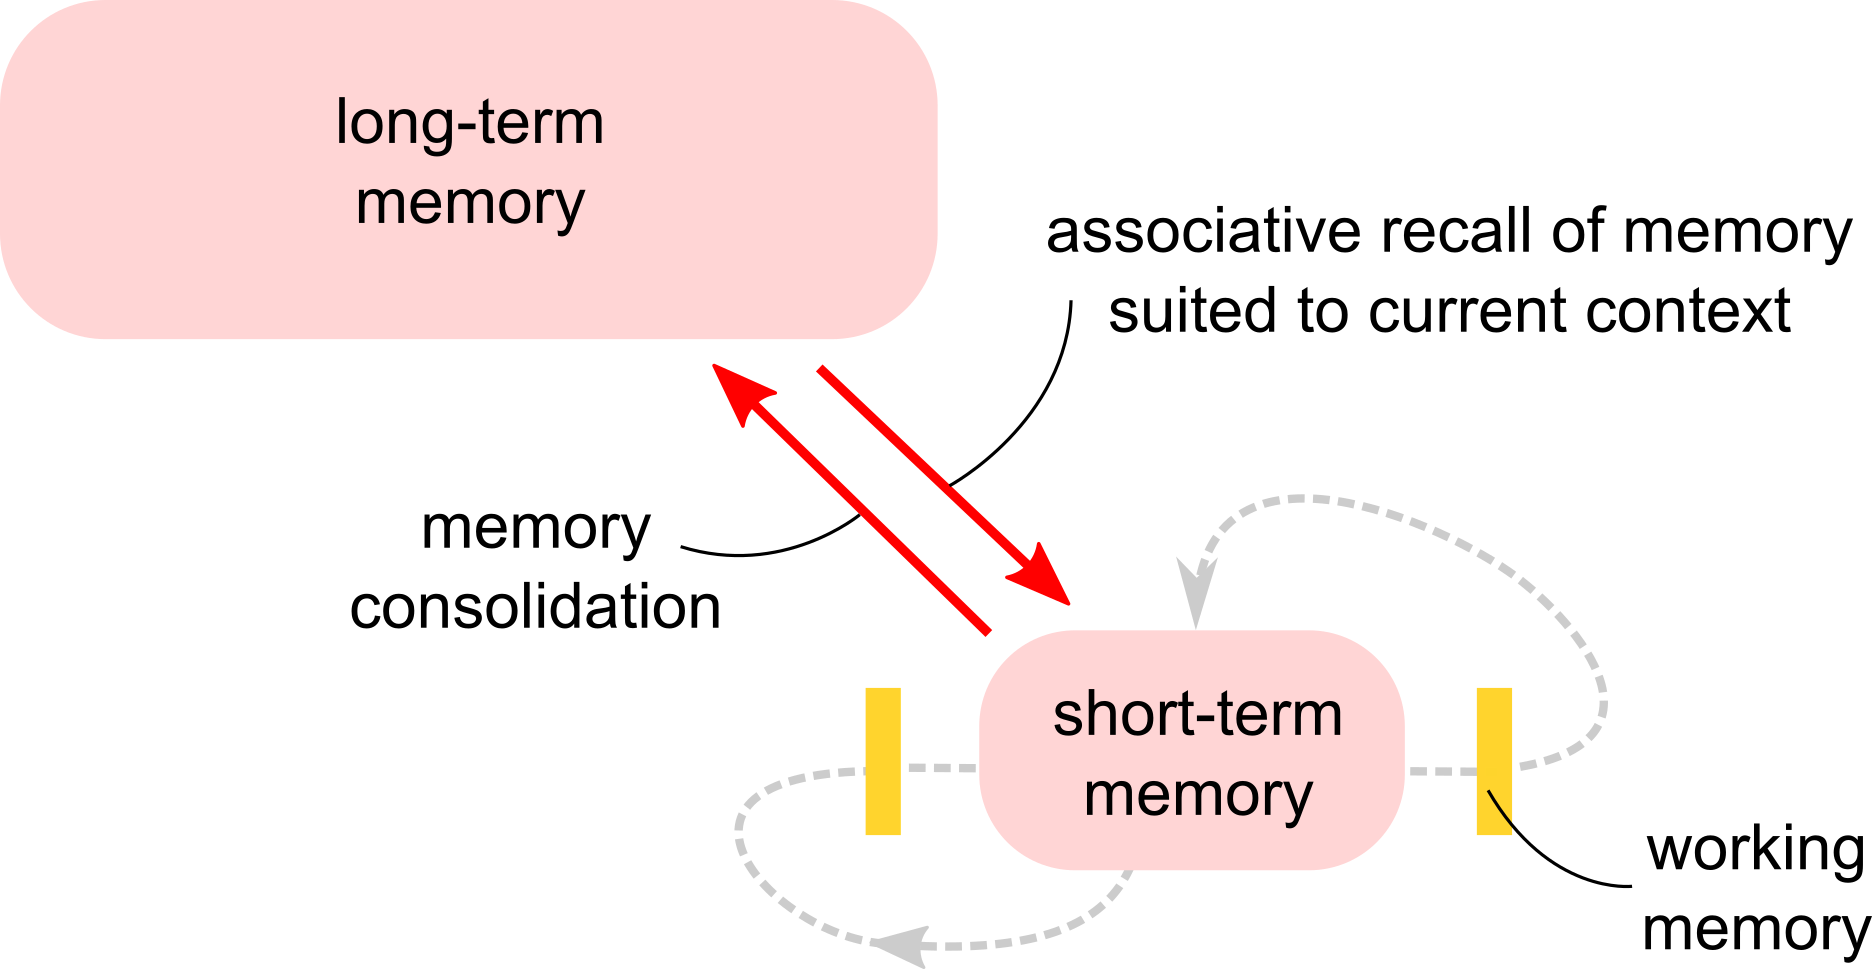
\includegraphics[scale=0.7]{memory-systems.png}}}
\end{equation}


\section*{Acknowledgements}

Thanks to David Ha and his co-authors for their PathNet idea.

\bibliographystyle{unsrtnat} % or number or aaai ...
\bibliography{AGI-book}

\end{document}
